\section{Introduction}
\label{sec:tutorial_introduction}

Swift Fox is an easy to learn programming language. It was designed to
allow the quick and easy deployment of a wireless sensor network (WSN)
running on top of the Fennec Fox platform \cite{marcin:whitepaper}. This
tutorial consists of two parts. The first part is titled ``\textit{Dive
Into Swift Fox}''\footnote{The title \textit{Dive Into Swift Fox} was 
inspired after the book \textit{Dive Into Python} by Mark Pilgrim
\cite{pilgrim:2004}.} and it has been written for novice Swift Fox
programmers, mostly contractors on the field who deploy a WSN and seek to 
customize its performance so as to meet their clients' needs. It describes
tools that are necessary to setup the network, and shows how to install
and configure them. Next, the Swift Fox language is taught step-by-step
through solving real life WSN deployment issues. In this part of the
tutorial we will follow Mike who is a contractor deploying WSNs. Based on
Mike's work we will demonstrate how a network is programmed using Swift
Fox.

The second part of the tutorial is titled ``\textit{Tune Up with Swift
Fox}''. This is the more advanced part of the tutorial written for expert
Swift Fox programmers who want to understand all the details of the
Swift Fox language. We will talk about typical errors, control flow, and
the compilation process. This part of the tutorial is a supplement to the
first part, which will allow a Swift Fox programmer to write correct code, 
understand errors, and debug programs.

\newpage
\section{Dive Into Swift Fox}

\subsection{Installation}
\label{sec:installation}

Swift Fox is a programming language that allows for the quick and easy
setup of self-reconfiguring WSNs. In order to be able to understand how to 
setup a network with Swift Fox, we first discuss the relationship between
the operating system (OS) running on the sensor nodes, Fennec Fox, and
Swift Fox.

WSNs are composed of sensor nodes, also known as motes, which are
severely restricted embedded devices \cite{culler:2004}. Similarly to other
embedded devices, sensor nodes require an OS to manage their resources and 
provide a hardware abstraction layer. Though some sensor networks may use
Linux, there is another special and lightweight OS designed for all sensor
motes, which we shall use. TinyOS is an operating system for WSNs in which 
we can execute simple applications that can run on the sensor network. On
top of the TinyOS we place the Fennec Fox platform. Fennec Fox is
essentially a middleware that allows sensor nodes to adapt the network
performance on the fly and also facilitates the development of adaptable
multi-tasking applications \cite{marcin:whitepaper}. Swift Fox is 
a programming language to configure the services provided by Fennec Fox.
The relationship between the underlying OS (\textit{e.g.,} TinyOS), Fennec 
Fox, and Swift Fox is illustrated in Figure \ref{fig:sflayers}. Using
Swift Fox we can easily program Fennec Fox to meet various system
objectives; Fennec Fox receives the blue-print of the expected network
performance, written in Swift Fox, and by using various protocols defined
in its libraries, it instructs the operating system to perform in a way
that will meet the programmers' expectations.

Evidently, to program a WSN with Swift Fox we will need to have a Swift
Fox compiler. However, because Swift Fox runs on top of the Fennec Fox,
which in turn runs on top of TinyOS, we will need to have these parts also
in place.

\begin{figure}[htp]
\centering
	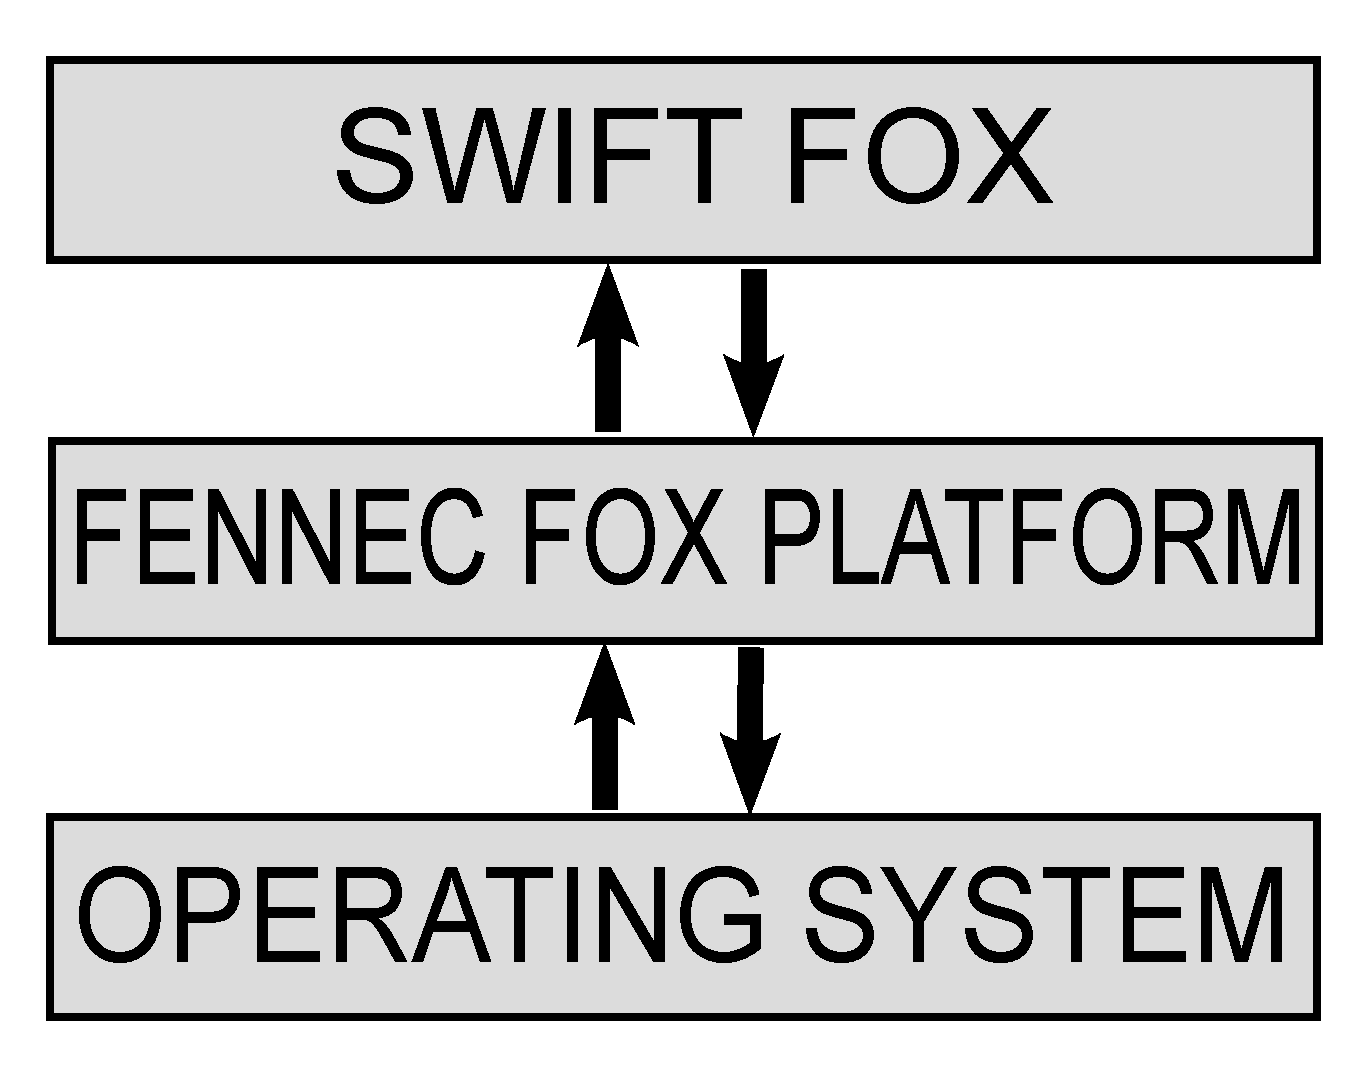
\includegraphics[scale=0.3]{fig/sflayers.eps}
	\caption{Swift Fox running on top of Fennec Fox}
	\label{fig:sflayers}
\end{figure}

The following components are necessary in order to successfully program a
WSN with Swift Fox:

\begin{enumerate}
	\item a laptop or a PC
	\item an OS for the WSN
	\item a running Fennec Fox platform
	\item a Swift Fox compiler
\end{enumerate}

Start by selecting some host machine, either a laptop or a PC, where you
can reserve some space to set up the Swift Fox programming environment.
This machine can either run Windows, Linux, or Mac OS X. However, in this
tutorial we recommend to use the VMware image prepared by the authors; any
machine with an OS that can run a VMware hypervisor should be fine
(\textit{e.g.,} VMware Workstation, VMware Player, or VMware Fusion).

TinyOS is the WSN OS that we will use. As we said before, Linux is another 
alternative for embedded devices such as wireless sensor motes, but it is
not yet supported by Fennec Fox. To prepare your machine to compile
programs written in Swift Fox, you will need to get TinyOS. One way of
installing TinyOS on your machine is by following installation steps as
explained on the TinyOS website: \url{http://www.tinyos.net}. It is
important to install correctly the TinyOS and nesC compiler, and setup the
system variables so as to compile Swift Fox programs. In the provided
VMware image, the TinyOS, nesC, C cross-compiler for ARM processors, 
and many other tools are already installed for you. This image can be
downloaded from: \url{http://www.cs.columbia.edu/~msz/wsn/}.

At this point we assume that you have either correctly installed TinyOS as
described on the TinyOS website, or you have downloaded the VMware image
from author's website. The next step is to install the Fennec Fox platform.
Fennec Fox can be downloaded from \url{http://www.cs.columbia.edu/~msz/fennec/}.
The current version is 0.03. After downloading, please install Fennec Fox 
into \texttt{/opt/fennec-0.03}.   

After the Fennec Fox installation ensure that the
\texttt{FENNEC\_FOX\_LIB} system variable is set correctly. If the
library path of the Fennec Fox was not changed during the installation
process, after running:	\\
\\
\texttt{\$ echo \$FENNEC\_FOX\_LIB}					\\
\\
from command line, one should get:					\\
\\
\texttt{/opt/fennec-0.03}						\\

Finally, the last thing you need is to get the Swift Fox compiler. You can
download the Swift Fox compiler from 
\url{https://nslvm2.cs.columbia.edu/trac/attachment/wiki/WikiStart/swift0.01.tar.gz}. 
Make sure that your Swift Fox compiler is on your system path, by running
\textbf{sfc}, which should print the Swift Fox welcome banner and a
description of how to use the compiler.

\texttt{\\
\\
\hspace*{4cm} Swift Fox Compiler!\\
\\
For example if you have a code in sample.sfc and library in sample.sfl, then run:\\
\\
\$ ./sfc sample\\
\\
}

Great! You have setup your computer to work with Swift Fox. Now, let us
introduce you to Mike.


\subsection{This is How We Do (step-by-step)}

Mike lives in Brooklyn and works as a network engineer for various
companies around New York City. Mike also has its own small business that
specializes in deployment, installation, and management of wireless sensor 
networks. Recently, he learned about Swift Fox. In his opinion, Swift Fox
can speed up and improve the quality of his work. We will spend a day with 
Mike to see how his typical work day looks like and why Swift Fox is
beneficial for him.

\subsubsection{Blinking}

Today Mike has a couple of WSNs to deploy. However, before deploying them
he is going to check if the hardware works correctly. It is possible that
during the shipment, some of the motes were broken. The simplest way to
verify that nothing is wrong with the motes is to order them to do a simple
task. Each mote has few light-emitting diodes (LEDs); Mike tests his motes 
by writing a program that orders them to start blinking one of their LEDs.

Mike's favorite text editor is \textit{vi}. Therefore, he invokes it and
starts programming the sensor motes as follows:				\\
\\
\texttt{\$ vi blink.sfp}						\\
\\
Of course Mike is free to use any editor he wants, apart from vi, in
order to create, edit, and save files. Inside the new file, Mike enters:\\ 
\\
\texttt{
configuration hello \{Blink nothing\}					\\
start hello								\\
}
\\
and then saves and closes the file. This simple program stored in the
\textit{blink.sfp} file can be compiled, resulting in code for Fennec Fox.
To compile blink.sfp program Mike enters in the shell:			\\
\\
\texttt{\$ sfc blink.sfp}						\\
\\
By calling \textbf{sfc}, Mike invokes the Swift Fox compiler. This 
compiler takes as the input the source code of a Swift Fox program. Once
the program is compiled, the generated Fennec Fox code together with
the operating system running on sensor motes (\textit{i.e.,} TinyOS) are
compiled to hardware dependent machine code, creating a new system image.
Mike wants to use the TinyOS operating system and to test blink.sfp on the 
telosB motes (\textit{i.e.,} a specific wireless mote brand). To compile
and install he should enter into a shell the following:			\\
\\
\texttt{\$ make telosb install}						\\
\\
This command will compile the code, load it into a telosb mote attached to 
Mike's laptop (or PC) through a USB port, and start the sensor mote. Mike
takes each mote, one by one, and loads the code into them. If the mote LED 
does not start blinking, then the mote is broken.

While Mike is testing his motes, let us discuss the Swift Fox program that 
he wrote. First, notice that this program is very short; it contains only
two lines. Mike's job is very simple: to check that motes can blink,
therefore his program should also be short and simple. Let us now dig into 
the code to understand what Mike has written there. The first line of the
program is:								\\
\\
\texttt{configuration hello \{Blink nothing\}}				\\

In this short statement, Mike defines the configuration of the 
wireless sensor network mote. To do this, he is using the keyword
\textbf{configuration}, which tells Swift Fox that whatever comes on the
right of the \texttt{configuration} keyword defines a system configuration.
The next word, which in Mike's program is \texttt{hello}, allows Mike to
give a name to the configuration that he defined. We do not know yet what
is the configuration, but we do know that Mike is defining one, and he is
calling this configuration \texttt{hello}. What comes next in the brackets 
is the definition of the configuration. The first word specifies the job
that the sensor mote should do, whereas the second word specifies the
communication mechanism that the sensor mote should use in order to
communicate with other motes. In this program, Mike tells the sensor motes 
to start blinking, by using the word \texttt{Blink}. He is also telling
the sensor motes not to use any kind of communication mechanism; he is
expressing this by using the word \texttt{nothing}. He does not want sensor
motes to send any messages. All he wants is to make sure that they are not 
broken, and he can check that by making their LEDs blink.

The second line of Mike's program is:					\\
\\
\texttt{start hello}							\\

In this statement Mike specifies the default configuration of the sensor
mote, right after it starts (boots up). To do this, Mike is using the
keyword \textbf{start} followed by the name of the configuration that he
has defined in the first line of the blink.spf program. In other words, the
second line of the program tells the motes to start running a configuration
called \texttt{hello}. Based on the definition of the \texttt{hello}
configuration, motes start executing the task, which is called
\texttt{Blink}, and they do not attempt to communicate since \texttt{hello}
configuration specifies \texttt{nothing} in the second field of the
definition.

Mike has finished testing all sensor motes and he puts them into his car.
Now we are ready to drive with Mike to the first site, where Mike will
demonstrate the commercial deployment of a WSN using Swift Fox. 

\vspace{\fill}

\subsubsection{Exercise}

The two line blinking test program written by Mike is actually not 
the simplest code you can write. Write a simpler two line Swift Fox 
program that will tell the sensor motes not to use any application 
or any communication mechanism.


\subsubsection{It's hot here, not!}

Mike's first client is Tony. Tony owns few buildings in Brooklyn and he is 
leasing apartments. Most of his buildings are around the Bay Ridge area
where he lives, but he also has a four-family building in Sunset Park. Last
winter was very cold and windy, so the temperature inside the buildings was
very low and required constant heating. Whenever it was cold, Tony had to
visit all his buildings to turn on the boilers. However, one day there was 
so much snow on the street that he could only walk to nearby buildings, but
he could not get on Sunset Park. People living in Tony's Sunset Park
building were freezing in their apartments, and Tony was violating The City
Housing Maintenance Code and State Multiple Dwelling Law that requires
building owners to provide heat and hot water to all tenants
\cite{nyc-dhpd:online}. Tony decides to invest in WSN technology, hoping
that Mike can setup a system that will automatically adjust the temperature
according to the New York City (NYC) regulations.

The NYC Department of Housing and Preservation Development specifies the
temperature requirements that should be met by the owners of NYC buildings 
\cite{nyc-dhpd:online}. According to these rules, between October 1st and
May 31st, temperature inside an apartment is required to be above 68 and 55
degrees Fahrenheit, between 6 AM till 10 PM and 10 PM till 6 AM
respectively. To make sure that temperature is never falling below the
value required by the city, and to make tenants feel warm inside their
apartments, Tony tells Mike to set the threshold values to 70 and 60
degrees Fahrenheit, for day and night respectively.

Mike starts designing his network with the specification of policies, which
will govern a network behavior that meets Tony's expectations. The wireless
sensor network, which Mike will deploy inside Tony's building, should
monitor the temperature all day and night, and send messages to the
boiler whenever temperature falls below the threshold values. On a piece of
paper, Mike draws a finite state machine, which will represent the various 
states of the network. His drawing is shown in Figure \ref{fig:fsm}.

\begin{figure}[htp]
\centering
	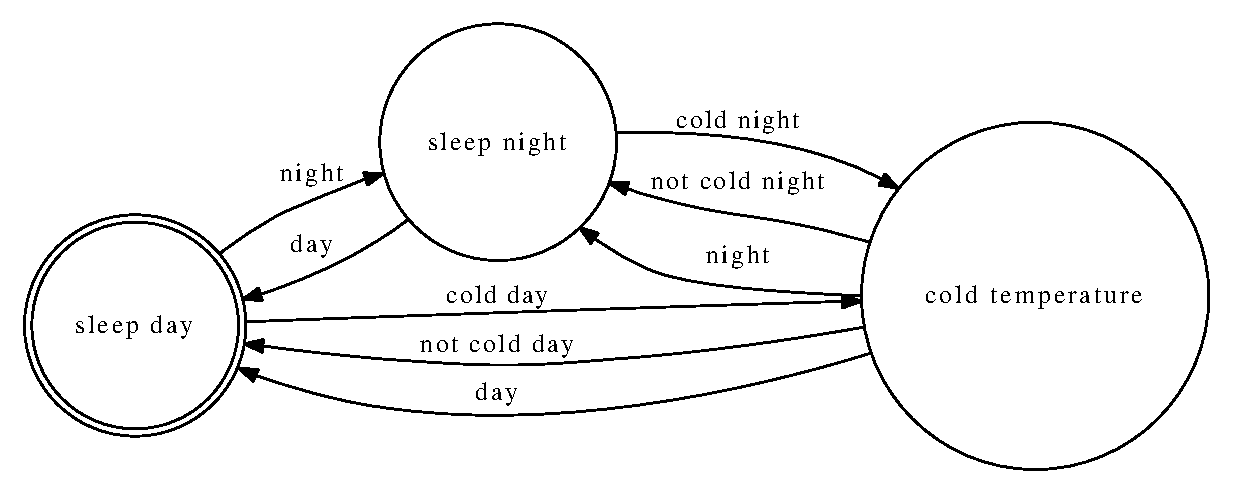
\includegraphics[scale=0.6]{fig/fsm.eps}
	\caption{Mike's drawing of the WSN states for Tony's building.}
	\label{fig:fsm}
\end{figure}

Based on the drawing, shown on Figure \ref{fig:fsm}, Mike comes to the
conclusion that his network has to operate in three different
configurations:								\\

\begin{enumerate}
	\item sleep during the day and monitor temperature
	\item sleep during the night and monitor temperature
	\item send temperature alerts when is too cold
\end{enumerate}
Mike opens a new file, called \textit{tony-bld.sfp}, and programs the 
following configurations in Swift Fox:					\\
\\
\texttt{
configuration sleep-day \{nothing CTP\}  				\\
configuration sleep-night \{nothing CTP\}				\\
configuration too-cold \{Send-Temp CTP\}				\\
}\\
Let us look at Mike's configuration definitions in more detail. He defines 
three configurations, which he calls according to the states of his drawing
(see Figure \ref{fig:fsm}). The names of these configurations are:
\textit{sleep-day}, \textit{sleep-night}, and \textit{too-cold}. In each of
these states there is network protocol activated, called \textit{CTP}. CTP,
which stands for Collection Tree Protocol, is the wireless sensor network
protocol that establishes a tree network topology, and can efficiently
collect data from sensor motes. Mike enables this protocol in all
configurations, even those that represent sensor motes in sleeping states
(\textit{i.e.,} motes that will not generate any alarm message). He wants
all motes to be able to send messages. In case one node senses low
temperature and starts sending temperature messages to the boiler, then
these messages would have to be forwarded through other sensor motes that 
are sleeping and not sensing the cold temperature. 

Once the configurations are defined, Mike starts defining events that will
trigger transitions between different configurations. Mike starts with two 
simple events: night and day, which will keep track of when the day and the
night start. To program this in Swift Fox he writes:			\\
\\
\texttt{
event-condition day \{Timer = 16hr\}					\\
event-condition night \{Timer = 8hr\}					\\
}\\
These two lines define two event-conditions. Each line starts with the
keyword \textbf{event-condition}, which says that what will follow is the
definition of a new event that is triggered when some condition becomes
true. In particular, the first line defines an event that is called
\textit{day}. This event uses a timer to measure time and is triggered
after 16 hours. Mike sets this event to 16 hours, because this is how long 
the sensor motes should measure temperature inside the building and test it
against the 70 degrees temperature value, which is the minimum temperature 
value that Tony is allowed to have inside the building during day
hours. Similarly, the second line defines an event called \textit{night},
which sets a timer for 8 hours.

By looking Figure \ref{fig:fsm} again, we notice that Mike has already
defined two events \textit{day} and \textit{night} that trigger network
reconfiguration and transition from one configuration to another. However, 
there are two more transitions related two the temperature; they are called
\textit{cold-day} and \textit{cold-night}. Mike programs them as follows:\\
\\
\texttt{
event-condition cold-day \{Temperature < 70F \}				\\
event-condition cold-night \{Temperature < 60F \}			\\
}\\
As before, these two new events have names: \textit{cold-day} and
\textit{cold-night} respectively. Both of these events are tested against
temperature sensing values, and their conditions are set to less than 70
and less than 60 degrees Fahrenheit. As in case of the two time related
events before, these two definitions of temperature related events have
similar constructs: the keyword \textbf{event-condition} is followed by a
chosen name of a new event definition, followed by a specification of the
source of event and a value condition applied to the data received from the
source of event.

Once configurations and events are defined, Mike specifies the policies
that will define the transitions between different configurations. First,
Mike notices that there are events, which they always trigger the same
configuration. These events are \textit{day} and \textit{night}. As shown
on Figure \ref{fig:fsm}, whenever \textit{day} occurs, the network is
reconfigured to the configuration called \textit{sleep-day}, and whenever
\textit{night} occurs, the network is reconfigured to the configuration
called \textit{sleep-night}. Mike programs these policies in Swift Fox as
follows:								\\
\\
\texttt{
from any goto sleep-day when day					\\
from any goto sleep-night when night					\\
}\\
Let us look at the first line of the code. This line creates a policy which
says whenever (the network can be at any configuration, as indicated by
keyword \textbf{any}) an event called \textit{day} occurs, reconfigure the 
network (expressed by keyword \textbf{goto}) to a configuration called
\textit{sleep-day}. Similarly, the second line creates a policy, which says
that whenever an event \textit{night} occurs, reconfigure the network to a 
configuration called \textit{sleep-night}. Policies in Swift Fox match
configurations and events together. 

All policy statements are specified by defining a transition from one, or
more, configurations to another configuration in the presence of an event.
Each policy starts with keyword \textbf{from}, which is followed by the
name of a configuration that is already defined. Hence, in Mike's case he
can start policies by writing the keyword \textbf{from} followed by
\textit{sleep-day}, \textit{sleep-night}, or \textit{too-cold}, which are
all configurations that he defined. The keyword \textbf{from} followed by
the name of the configuration says that this policy can only be considered 
when the network is currently configured according to that configuration
name. Therefore, if the network is currently in configuration
\textit{sleep-day}, none of the policies starting with \textbf{from}
\textit{sleep-night} or \textbf{from} \textit{too-cold} can be applied. The
exception to this rule is a policy starting with \textbf{from}
\textbf{any}, which always has to be applied, no matter what is the current
configuration of the network. Next, we have a policy statement that is
followed by the keyword \textbf{goto} and another configuration name; one
of those already defined. The \textbf{goto} $<configuration-name>$ part of 
the policy statement specifies the configuration in which the network
should be after the policy is applied. For example, Mike may say
\textbf{from} \textit{sleep-day} \textbf{goto} \textit{sleep-night}, which 
starts a policy that is considered when the network is in configuration
\textit{sleep-day} and when it is applied, leaves the network in
configuration \textit{sleep-night}. Finally, the policy statement ends with
the event that must be fired to trigger the network reconfiguration. This
last part of the policy statement starts with the keyword \textbf{when} and
it is followed by an event name that is already defined. For example, Mike 
can say \textbf{when} \textit{day} or \textbf{when} \textit{cold-night}.
All defined events can also be used in negation by preceding the event name
with keyword \textbf{not}. For example, Mike is using negation on his
transition events in Figure \ref{fig:fsm}, where he says
\textit{not cold-day} and \textit{not cold-night}. Let us actually see how 
does he program the rest of the events, that are related to the temperature
conditions.								\\
\\
\texttt{
from sleep-day goto too-cold when cold-day				\\
from sleep-night goto too-cold when cold-night				\\
from too-cold goto sleep-day when not cold-day				\\
from too-cold goto sleep-night when not cold-night			\\
}									\\
Up to this point it should be straightforward to understand Mike's
policies, but let's go once more over the last policy. The last policy is
only considered when the network is in configuration \textit{too-cold}. If 
that is true, the \textbf{not} occurrence of the event called
\textit{cold-night} is checked. Note that if it is actually cold, and the
event \textit{cold-night} is triggered, this policy is skipped. However, if
it is not cold, meaning that the event \textit{cold-night} is not
triggered, the policy is applied, which means that the network is
reconfigured to the \textit{sleep-night} configuration. 

After defining all configurations, the events, and then specifying
the corresponding policies, Mike has to write one more statement; the
initial configuration statement. For this program Mike writes:		\\
\\
\texttt{
start sleep-day								\\
}

Mike adds comments inside the program code and saves his program in 
a \textit{tony-bld.sfp}. Comments start with the hash (\#) symbol. 
Everything that Mike writes on a line that starts with \# is not 
a part of the program, and the Swift Fox compiler will skip it. 
The comment lines are useful for
documenting the code and for noting important information.

\vspace{\fill}

\subsubsection{Exercise}

Before we move to the other examples of the programs written by 
Mike, for one more time consider the tony-bld.sfp program and 
the associated Figure \ref{fig:fsm}. Based of the figure and 
the code, can you tell when (at what hour) Mike will start (boot up)
the sensor network to collect the temperature readings 
inside of the Tony's building on the Sunset Park?

\newpage
The complete Swift Fox code for the temperature monitoring system that Mike
will install in Tony's building is the following:			\\
\\
\texttt{
\# tony-bld.sfp								\\
\# Author:   Mike							\\
\# Date:  03/12/2010							\\
\# Job:  Tony's building on Sunset Part					\\
\# Program:  Monitor temperature and send data to boiler 		\\
\\
\# define configurations 						\\
\\
configuration sleep\_day \{nothing nothing\} 				\\
configuration sleep\_night \{nothing nothing\}				\\
configuration too\_cold \{sendTemp ctp\}				\\
\\
\# define time passing events						\\
\\
event-condition day \{timer = 16hr\} 					\\
event-condition night \{timer = 8hr\}					\\
\\
\# define temperature sensing events					\\
\\
event-condition cold\_day \{temperature < 70F \}			\\
event-condition cold\_night \{temperature < 60F \}			\\
\\
\# reconfiguration policies						\\
\\
from any goto sleep\_day when day					\\
from any goto sleep\_night when night					\\
from sleep\_day goto too\_cold when cold\_day				\\
from sleep\_night goto too\_cold when cold\_night			\\
from too\_cold goto sleep\_day when not cold\_day			\\
from too\_cold goto sleep\_night when not cold\_night			\\
\\
\# and finally, the initial configuration				\\
\\
start sleep\_day							\\
}

\newpage

The library file for Tony's building would be saved in tony-bld.sfl file
and would contain the following libraries:				\\
\\
\texttt{
\# Standard Fennec Fox Applications					\\
\\
use application blink \$(FENNEC\_FOX\_LIB)/Application/SimpleBlink	\\
use application collector \$(FENNEC\_FOX\_LIB)/Application/DataCollector\\
use application sendTemp \$(FENNEC\_FOX\_LIB)/Application/SendTemp	\\
\\
\# Standard Fennec Fox Network Protocols				\\
\\
use network broadcast \$(FENNEC\_FOX\_LIB)/Network/broadcast		\\
use network ctp \$(FENNEC\_FOX\_LIB)/Network/ctp			\\
\\
\# Events								\\
\\
use source temperature \$(FENNEC\_FOX\_LIB)/Events/Temperature		\\
use source timer \$(FENNEC\_FOX\_LIB)/Events/Timer			\\
}

\newpage

\section{Tune Up with Swift Fox}

\subsection{Errors and Exceptions}

Beginners writing in a new language often make errors and mistakes. These
errors may confuse or carry an incorrect message. Although Swift Fox is a
relatively simple programming language, with limited number of keywords and
constrained structure, initial programming in Swift Fox can be error prone.
To minimize the number of errors, which in Swift Fox can be typographical
or syntactical, the Swift Fox compiler has a mechanism to catch language
errors and exceptions.

Swift Fox errors and exceptions mechanisms are designed to provide
readable and intuitive feedback to the programmer and to ensure the correct
execution of the underlying Fennec Fox platform. Programs written by novice
Swift Fox programmers may contain a lot of errors. During compilation,
Swift Fox recognizes an error, and provides a descriptive error message to
the programmer, along with a hint about its possible source and a way of
recovering. Swift Fox reports errors related to one statement at the time
only, and aborts. If there are more errors in the following program
statements, these errors will be reported after the first error line is
corrected and accepted by the compiler during the next compilation
process.								

For example, we may have a program that starts with two configuration
statements, where the second statement is missing left bracket '\{': \\
\\
\texttt{configuration report \{ collector ctp \} \\
configuration sleep  nothing nothing \}\\
}
%configuration sleep  nothing nothing \}}\\

\noindent When this program is compiled Swift Fox reports the following 
error message which displays the error line and indicates the position
of the error within the line. Swift Fox compiler will also specify if
the source of the syntax error is in the library or in the program file.\\
\\
\texttt{\$ sfc example\\
\\
sfc in program: example.sfp\\
syntax error at 2 in this line:\\
configuration sleep  nothing nothing \}\\
\hspace*{4cm}\^\\
}

\subsection{Control Flow}
\label{sec:control}

The control-flow statements of the Swift Fox language specify the order in 
which configuration and events are defined, and the priority and order in
which the execution of policies is performed. In the first part of the
tutorial all types of statements were presented and the flow of the program
was discussed based on Swift Fox examples. Now, the control flow will be
presented in a more formal way.

All Swift Fox programs have a fixed and well defined structure. First, a
Swift Fox program starts with at least one or more configuration definition
statements. Formally, the syntax of a configuration statement is:	\\
\\
\texttt{\textbf{configuration} \textit{configuration-name} 
  \{ \textit{list-of-component-names} \} }	 			\\
\\
where the \textit{list-of-component-names} in the current version of the
Swift Fox is a list of two components, one for the application task and one
for the network protocol, which together construct a definition of a new
Fennec platform configuration. Second, following the configuration
statements, Swift Fox programs have zero or more event definition
statements. Formally, the syntax of the event statement is:		\\
\\
\texttt{\textbf{event-configuration} \textit{event-name} 
  \{ \textit{event-condition} \} }					\\
\\
where the \textit{event-condition} consists of the source of the event
followed by a relational operator and the constant value that specifies the
condition to be met. Third, after the event statements, Swift Fox programs 
have zero or more policy definitions. Formally, the syntax of the policy
definition is:								\\
\\
\texttt{\textbf{from} \textit{configuration-name} \textbf{goto} 
  \textit{configuration-name} \textbf{when} \textit{event-name} }	\\
\\
where the first \textit{configuration-name} is a name of already defined
configuration according to which Fennec Fox has to be configured to
consider this policy valid. A policy that is universally valid, meaning a
policy that should always be considered no matter what is the name of the
current configuration, should use a special keyword \textbf{any}. The
second \textit{configuration-name} should be an already defined
configuration to which the system should be reconfigured in the presence of
the \textit{event-name} event. Policies are applied from top to bottom, and
once the policy condition becomes true, the system is reconfigured
according to the configuration specified in the second
\textit{configuration-name}. Finally, Swift Fox programs have a one-line
initial configuration statement. Formally, the syntax of this statement is:\\
\\
\texttt{\textbf{start} \textit{configuration-name} }			\\
\\
where the \textit{configuration-name} is the name of the defined
configuration in which Fennec Fox starts after system is booted.

Concluding, control flow in Swift Fox is top to bottom, without any 
statements that would alter it. Comparing to other languages like C, Java, 
and Python, there are no if-else statements, while loops, gotos, and
labels. Because of this, Swift Fox programs are readable, from top to
bottom, allowing for a intuitive and easy to understand programming style, 
with the declarations of configurations and events preceding the
specification of polices.


\subsection{Run-Time Environment}
\label{sec:runtimeenv}

The Swift Fox compiler generates code that corresponds to a Swift Fox
program and runs it on the Fennec Fox platform. Once the system environment
is created, it stays fixed afterwards. From the perspective of the Swift
Fox programmer, everything that is defined is globally accessible, so once 
a configuration, or an event is defined, it can be used in the rest of the 
program. The Fennec Fox run-time environment needs to be fixed for various
reasons, but more importantly for assisting the memory and storage
allocation, access to variables, and linkage between the various Fennec Fox
components, which are actually taken care by the run-time environment of
the system in which Fennec Fox is executed. For example, the issues
previously listed, are taken care by TinyOS and nesC compiler, or Linux and
C compiler, depending on the OS that hosts Fennec Fox.

Swift Fox uses libraries, as well as configuration and event declarations
to generate a run-time environment in Fennec Fox. The library source
definitions are used in order to locate libraries with platform components 
that provide various functionalities, such as applications, protocols, and
so forth. The source code stored in such libraries provides the services
requested in the configuration and event declarations. Notice that during
compilation, only services that are utilized are actually included in
Fennec Fox. For example, Swift Fox has a library with applications, and one
of them, Blink, provides a service with a simple task that blinks LEDs on
the sensor mote. If this task, Blink, is used in any of the configuration 
statements, the code of the Blink is included in the Fennec Fox, and Swift 
Fox can refer to this task from various statements in the code. Otherwise, 
although Swift Fox knows about Blink, it will not include its code inside 
the Fennec Fox, since this code is never used, and the Blink task will
not be accessible.


\subsection{Libraries}

Libraries contain source code that provides some service classified
according to the components of the Fennec Fox platform. For example,
libraries can provide application services, where simple tasks can be
called and executed (\textit{e.g.,} Blink). Libraries also contain code
related to services of other components, such as network protocols,
security, and quality of information. Currently, only libraries related to 
application tasks and network protocols are supported in Swift Fox. These
libraries can be part of the Swift Fox standard library or can be a third
party libraries. 

\subsection{Swift Fox Standard Library}

Swift Fox standard library is directly related to the Fennec Fox library,
which provides applications, network protocols, and other services
provided by the Fennec Fox platform. At the current state Swift Fox 
contains two simple libraries with applications and network protocols. The
application library contains three simple applications: blink that blinks 
LEDs, sendTemp that senses temperature and broadcasts the sensed temperature to a 
base station, and sendHum that senses humidity and broadcasts the sensed
humidity to a base station. The network library contains two protocols:
the Collection Tree Protocol, known as CTP, and a simple broadcast protocol.
Fennec Fox library also provides handle functions for event management.
At the current state timer, temperature, and humidity events have been 
ported to the Swift Fox. Timer event can be requested to fire after some 
period of time, whereas temperature and humidity events fire when
sensor's reading reaches specified threshold value.
Eventually, more applications, network protocols, and sources 
of events will be supported by Swift Fox standard library.

\subsection{Compilation}
\label{sec:compilation}

\begin{figure}[htp]
\centering
        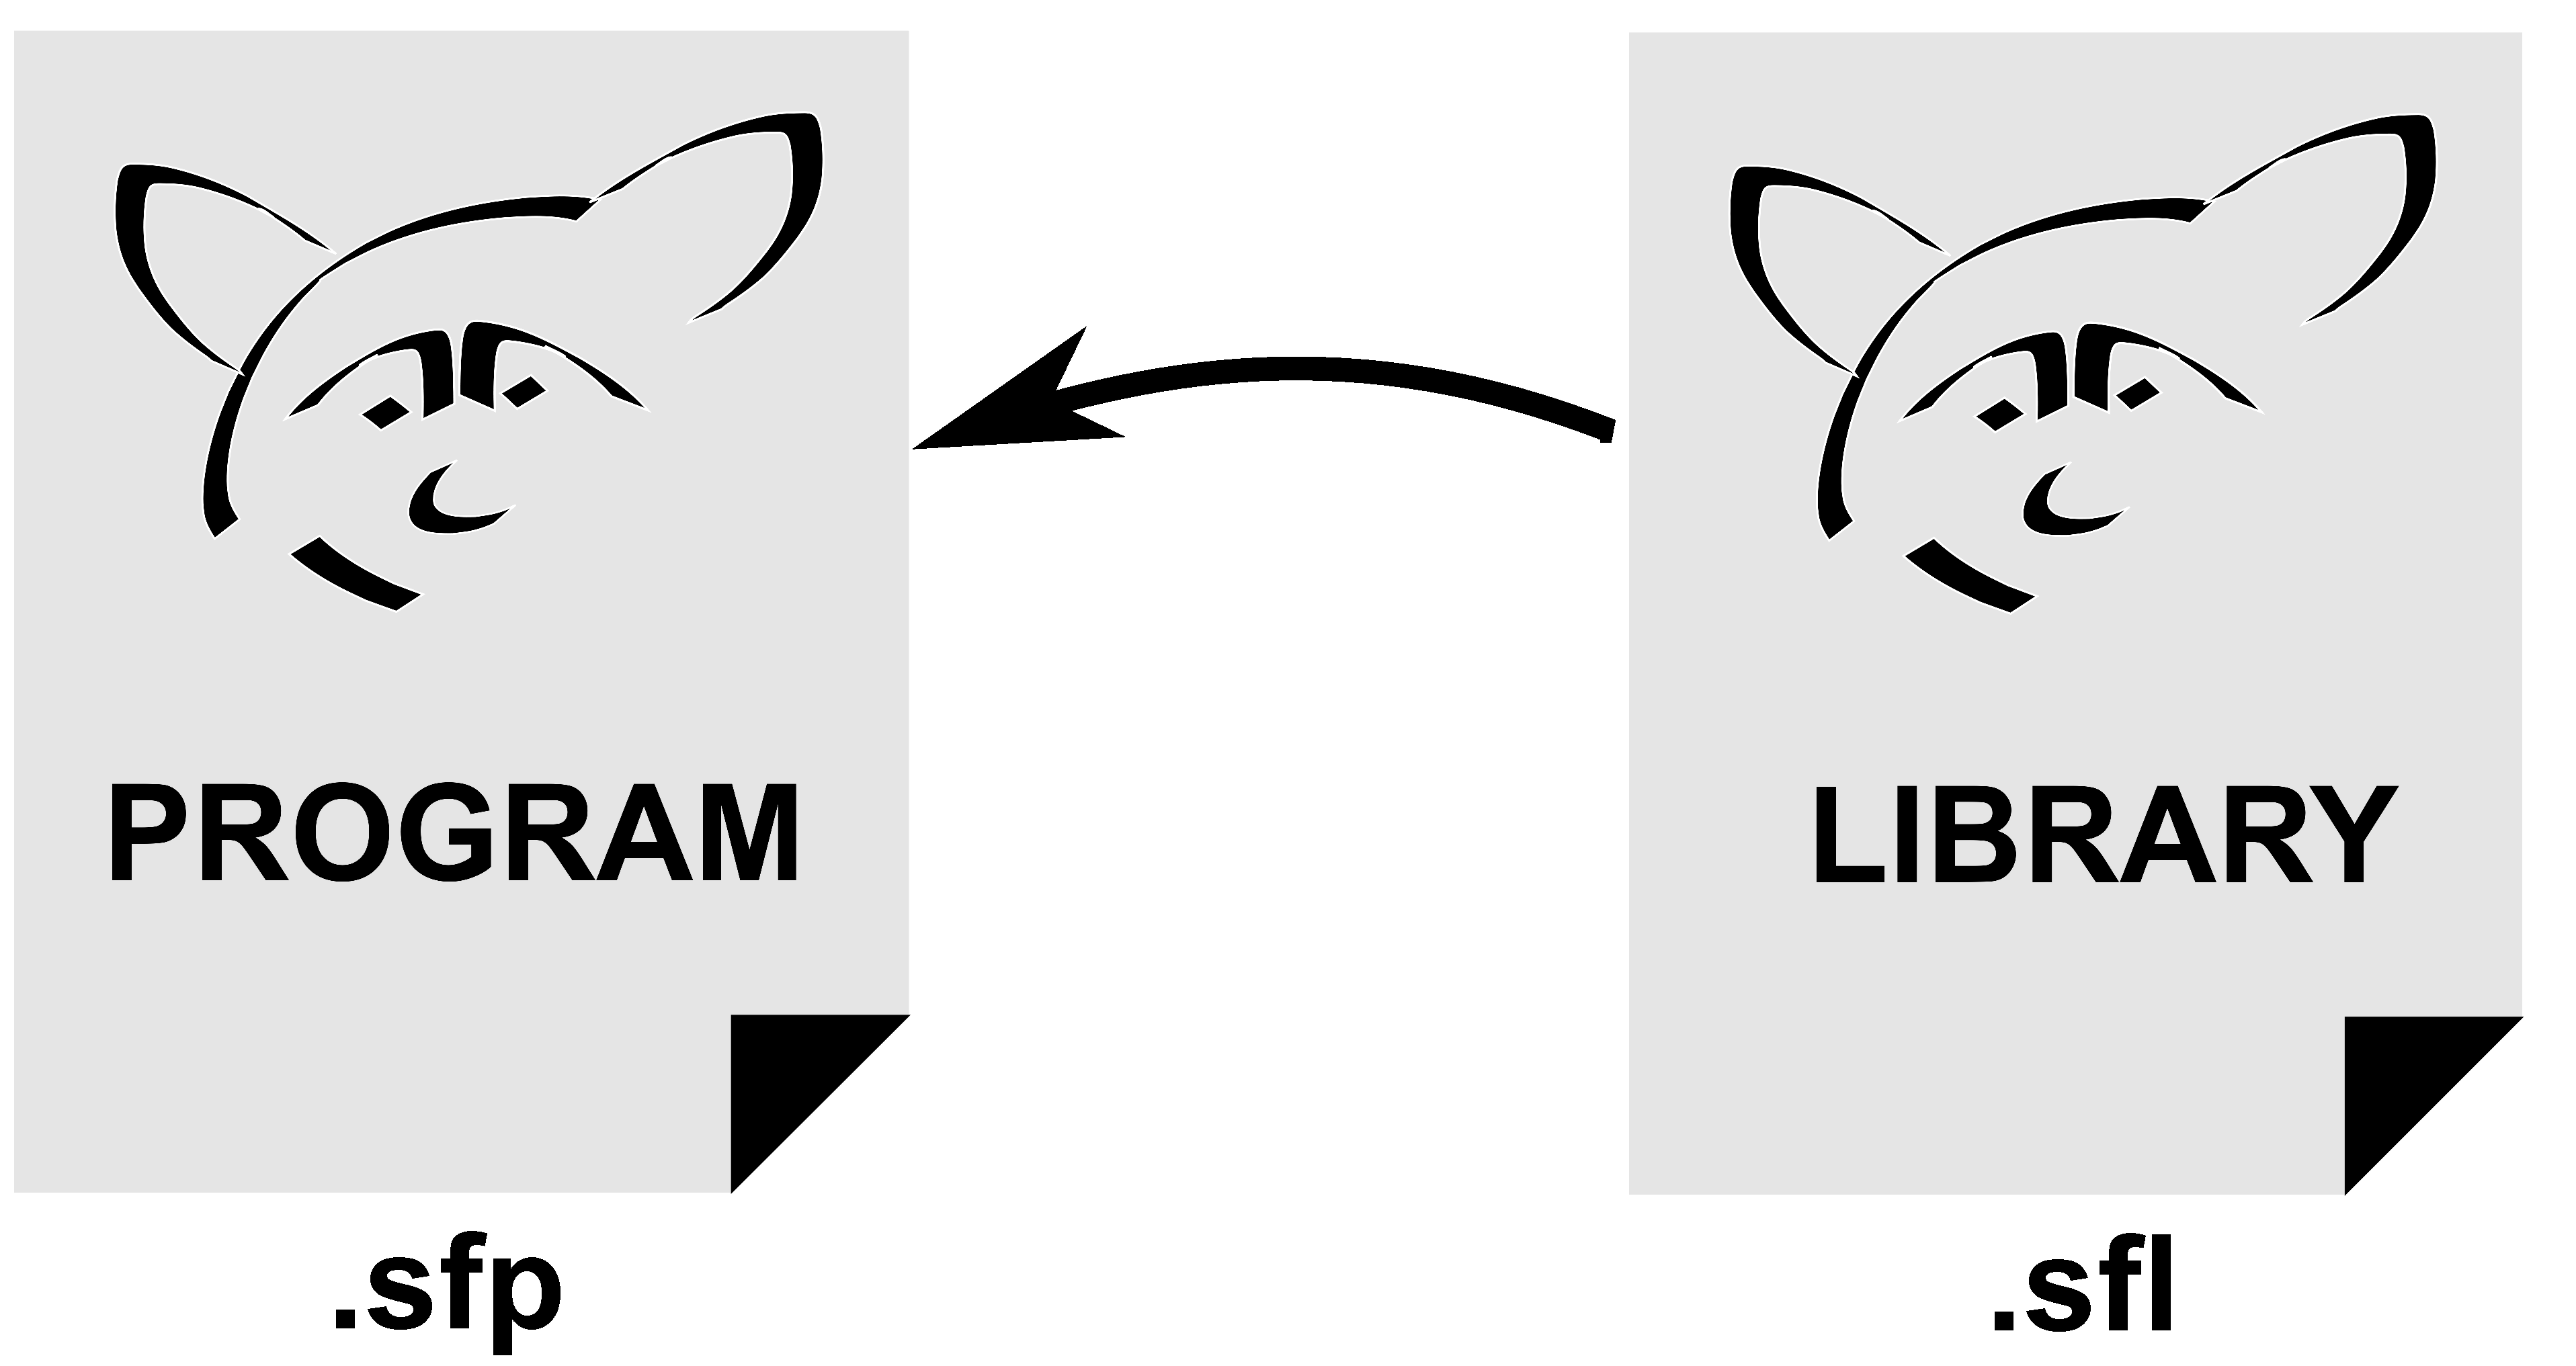
\includegraphics[scale=0.2]{fig/swift_fox_relation.eps}
        \caption{Swift Fox source files (.sfp) and libraries (.sfl)}
        \label{fig:swift_fox_relation}
\end{figure}

Swift Fox programs are compiled as follows:     			\\
\\
\texttt{sfc <program\_name>}	          				\\
\\
where \texttt{sfc} is the command to start the Swift Fox compiler, and
$<program\_name>$ is the path of the file containing the source code of the
program written in Swift Fox. Source code files must have the suffix
\texttt{.sfp}, which stands for Swift Fox Program. Before compilation, the
compiler looks for a special file specifying where libraries of various
Fennec Fox components are available. This allows the compiler to check if
all libraries used in policies written in the Swift Fox program exist and
are accessible to the compiler (\textit{e.g.,} where are all the
applications and network protocols specified inside the Swift Fox program).
Swift Fox looks for the library file in the current directory under the
name $<program\_name>.sfl$. Therefore, Swift Fox library files must have
the suffix \texttt{.sfl}, which stands for Swift Fox Library. 

Figure \ref{fig:swift_fox_relation} illustrates the relationship 
between a Swift Fox program and its corresponding library file. 
First Swift Fox compiler processes the library file, saving the path
to the source code of each library and labeling the library with
an appropriate type. For example, a library with \textit{blink} application 
has type \textit{application}. Next, Swift Fox compiles the program file.
During the compilation, Swift Fox uses information from library to
ensure that all types are correct and that program code refers only
to Fennec Fox services which path is known.



